\documentclass[pdf]{beamer}

\usepackage[T1]{fontenc}
\usepackage[utf8]{inputenc}
\usepackage[english, french]{babel}

\usepackage{xcolor, graphicx, shorttoc}

% ================================
%             STYLE
% ================================

% beamer
% theme
\usetheme{mcgill}

% nav
\setbeamertemplate{navigation symbols}{}


% ================================
%            COLORS
% ================================

% définition des couleurs pour la syntaxe
\definecolor{backcolor}{rgb}{0.85, 0.85, 0.85}
\definecolor{codebasic}{rgb}{0.3, 0.3, 0.3}
\definecolor{codeblue}{rgb}{0.2, 0.2, 0.9}
\definecolor{codecyan}{rgb}{0, 0.5, 0.8}
\definecolor{blush}{rgb}{0.87, 0.36, 0.51}
\definecolor{cardinal}{rgb}{0.77, 0.12, 0.23}
\definecolor{codeorange}{rgb}{1, 0.5, 0}
\definecolor{codegray}{rgb}{0.5, 0.5, 0.5}
\definecolor{codegreen}{rgb}{0, 0.6, 0}

% ================================
%            COMMANDS
% ================================

% commands
% ================================
%            COMMANDS
% ================================

% generic commands
\newcommand{\strong}[1]{\textbf{#1}}                    % highlight text
\newcommand{\langue}[1]{\textit{#1}}                    % text in another language
\newcommand{\citer}[1]{\og #1 \fg}                      % quote
\newcommand{\code}[1]{\texttt{#1}}                      % few one-line source code
\newcommand{\figureref}[1]{\textsc{Figure}~\ref{#1}}    % reference to a figure
\newcommand{\propre}[1]{\textsc{#1}}                    % proper name
\newcommand{\nom}[2]{#1 \textsc{#2}}                    % person name {first}{last}
\newcommand{\logo}[1]{\texttt{\textsc{#1}}}             % acronym

% report specific commands
\newcommand{\bibquote}[3]{\citer{#1}, \logo{#2}.\\\small\url{#3}\normalsize}
\newcommand{\anneeUniversitaire}{De Novembre 2024 à Février 2025}
\newcommand{\HRule}{\rule{\linewidth}{0.5mm}}
\newcommand{\univ}[1]{\textsc{Université Marie et Louis Pasteur}}
\newcommand{\ofni}{\logo{OFNI}}
\newcommand{\game}{\logo{Space OFNIvaders}}
\newcommand{\formwidget}{\logo{Form-Widget}}
\newcommand{\web}{\textsc{web}}


% ================================
%            PARAMETERS
% ================================

\title[Refonte du site internet de l'association]{Refonte d'un site internet pour une association étudiante}
\author[OFNI]{
    \nom{Tristan}{Amiotte-Suchet} \\
    \nom{Antoine}{Cuinet} \\
    \nom{Gaspard}{Quentin} \\
}
\institute{Université de Franche Comté}
\date{De novembre 2024 à mars 2025}
\logo{pictures/logo-umlp-black.png}

% ================================
%             DOCUMENT
% ================================

\begin{document}

% title page
\frame[plain, noframenumbering]{\titlepage}

% table of contents
\begin{frame}
    \frametitle{Plan de la présentation}
    \tableofcontents[hideallsubsections]
\end{frame}


% introduction
% @Antoine
\section{Le site de l'OFNI}
\sectitle{Le site internet de l'OFNI}

\begin{frame}
    \frametitle{Introduction}
    \centering
    \textbf{Objectif}: Concevoir et développer un nouveau site web pour l’OFNI
    \vspace{1cm}

    \textbf{Processus}: Analyse des besoins, maquettage, choix des technologies et implémentation des différentes fonctionnalités
\end{frame}

\begin{frame}
    \frametitle{Le site web de l’association OFNI}
    \centering
    \textbf{Trois phases}: Maquettage du site, développement du site et réalisation du rapport et de la soutenance orale
\end{frame}

\begin{frame}
    \frametitle{Le site web de l’association OFNI}
    \centering
    \textbf{OFNI}: Association des étudiants en informatique de l’université
    \vspace{1cm}

    \textbf{Pourquoi ce projet?} Ancien site obsolète, non mis à jour, failles de sécurité, ne répond plus aux besoins actuels
\end{frame}


% maquettage
% @Gaspard
\section{Maquettage}
\sectitle{Maquettage du site}

\begin{frame}
    \frametitle{Réflexions préliminaires}

    \begin{itemize}
        \item Définition des besoins du site (\textbf{réunions hebdomadaires}).
        \item Analyse des améliorations par rapport à l’ancien site.
        \item Étude de faisabilité en lien avec le \textbf{RGPD}.
    \end{itemize}
\end{frame}

\begin{frame}
    \frametitle{Les fonctionnalités du site}

    \begin{itemize}
        \item \textbf{Présentation de l’association} et de son histoire.
        \item \textbf{Gestion des événements} (inscriptions et suivi).
        \item \textbf{Page d’actualités}.
        \item \textbf{Boutique en ligne} (adhésion et produits).
        \item \textbf{Galerie photo}.
        \item \textbf{Espace administrateur} (gestion des événements, photos, etc.).
        \item \textbf{Système de comptes} (utilisateurs et administrateurs).
        \item \textbf{Jeu ludique} inspiré de \textit{Space Invaders}.
    \end{itemize}
\end{frame}

\begin{frame}
    \frametitle{Choix des technologies}

    \begin{itemize}
        \item Outil de gestion de projet : \textbf{Trello}.
        \item Serveur : choix d’un framework \textbf{PHP}.
        \item Comparaison \textbf{Laravel} vs \textbf{Symfony} :
              \begin{itemize}
                \item Laravel : approche fonctionnelle, plus simple mais moins familière.
                \item Symfony : approche orientée objet, plus adaptée à nos compétences.
              \end{itemize}
        \item Décision finale : \textbf{Symfony} pour sa maintenabilité et son usage répandu en France.
    \end{itemize}
\end{frame}

\begin{frame}
    \frametitle{Maquettage du site}

    \begin{itemize}
        \item Conception en \textbf{deux étapes} :
              \begin{itemize}
                \item \textbf{Esquisse manuscrite} pour organiser les pages.
                \item \textbf{Maquette numérique} réalisée sur \textbf{Figma}.
              \end{itemize}
        \item Validation et ajustements après échanges avec les tuteurs.
        \item Réflexion sur la maintenabilité (\textbf{gestion de contenu sans code}).
    \end{itemize}
\end{frame}

\begin{frame}
    \frametitle{Exemples de maquettes}

    \begin{minipage}{0.48\textwidth}
        \centering
        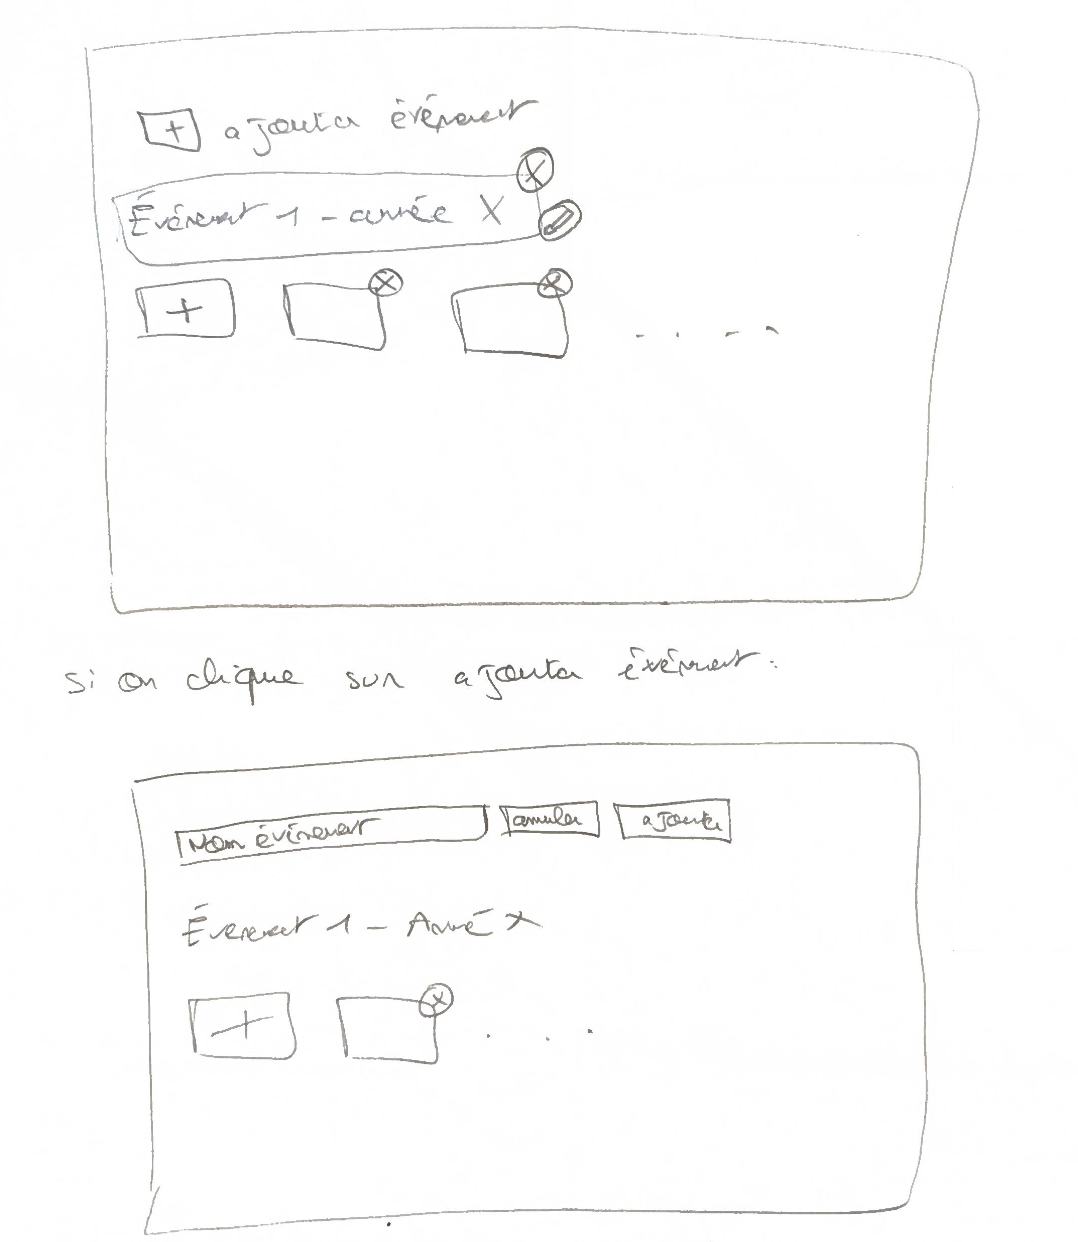
\includegraphics[width=\linewidth]{pictures/maquette.png}
        %\captionof{figure}{Esquisse manuscrite}
    \end{minipage}
    \hfill
    \begin{minipage}{0.48\textwidth}
        \centering
        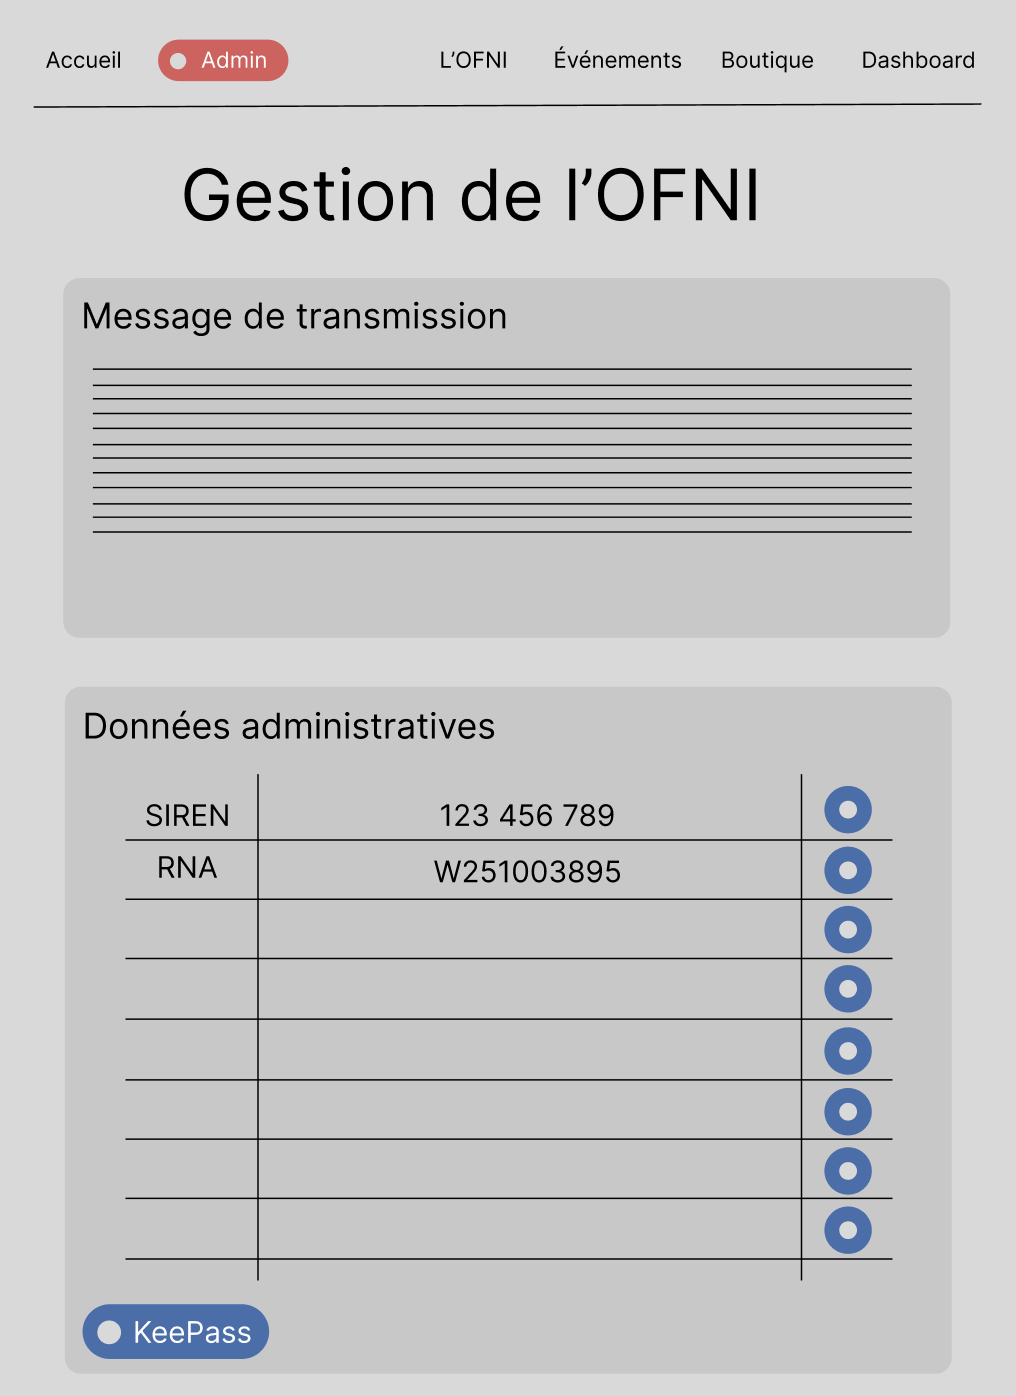
\includegraphics[width=\linewidth]{pictures/figma.png}
        %\captionof{figure}{Maquette numérique}
    \end{minipage}
\end{frame}


% implémentation
% @Gaspard
\section{Implémentation}
\sectitle{Implémentation du projet}

\begin{frame}
    \frametitle{Implémentation du site}

    \begin{itemize}
        \item Développement en \textbf{Symfony} (architecture MVC).
        \item Structuration du code :
              \begin{itemize}
                \item \textbf{Modèle} : gestion des données et BDD.
                \item \textbf{Vue} : affichage via \textbf{Twig}.
                \item \textbf{Contrôleur} : lien entre modèle et vue.
              \end{itemize}
    \end{itemize}
\end{frame}

\begin{frame}
    \frametitle{Architecture MVC}

    \centering
    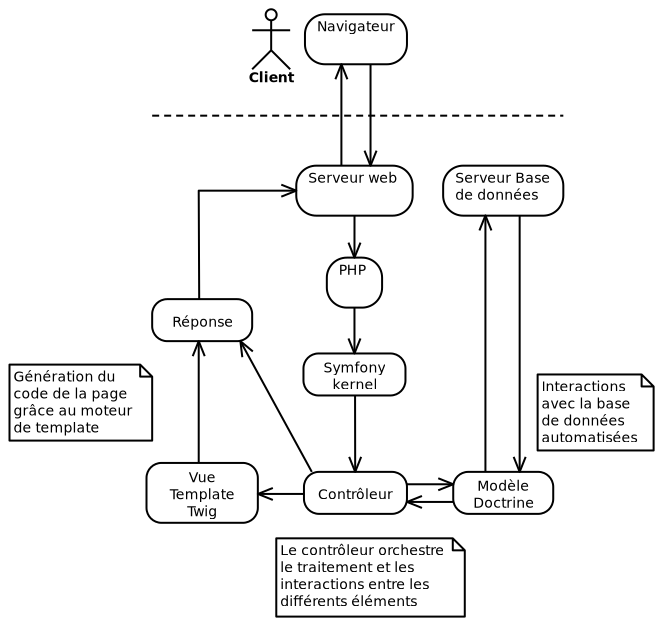
\includegraphics[width=0.7\linewidth]{pictures/mvc.png}
    %\caption{Architecture MVC dans Symfony}
\end{frame}

\begin{frame}
    \frametitle{Technologies utilisées}

    \begin{itemize}
        \item \textbf{Sass} : amélioration et structuration du CSS.
        \item Avantages de Sass :
              \begin{itemize}
                \item Variables et réutilisation de styles.
                \item Meilleure organisation du code CSS.
              \end{itemize}
        \item \textbf{JavaScript} : utilisé pour le jeu intégré au site.
    \end{itemize}
\end{frame}


% structuration
% @Tristan
\section{Structuration}
\sectitle{Structuration des données}

\begin{frame}
    \frametitle{Redondance des événements}
    Le constat :
    \begin{itemize}
        \item Événements redondants
        \item Informations dupliquées
    \end{itemize}
    \pause
    \vspace{2em}
    Notre choix :
    \begin{itemize}
        \item Événements fixes
        \item Nouvelle éditions chaque année
    \end{itemize}
\end{frame}

\begin{frame}
    \frametitle{Inexhaustion des formulaires}
    Le constat :
    \begin{itemize}
        \item Besoins spécifiques par événement
        \item Formulaires souvent similaires
    \end{itemize}
    \pause
    \vspace{2em}
    Notre choix :
    \begin{itemize}
        \item Formulaires personnalisables
        \item Construction récursive
    \end{itemize}
\end{frame}

\begin{frame}
    \frametitle{Gestion de la récurtion}
    Généralisation d'un formulaire $\Longrightarrow$ \textit{\textbf{FormWidget}} \\
    \pause
    \vspace{3em}
    3 types de \textit{FormWidget} :
    \begin{itemize}
        \item<3-> Natif
        \item<4-> Composite
        \item<5-> Liste
    \end{itemize}
\end{frame}

\begin{frame}
    \frametitle{Structure finale de la base de données}
    \begin{figure}
        \centering
        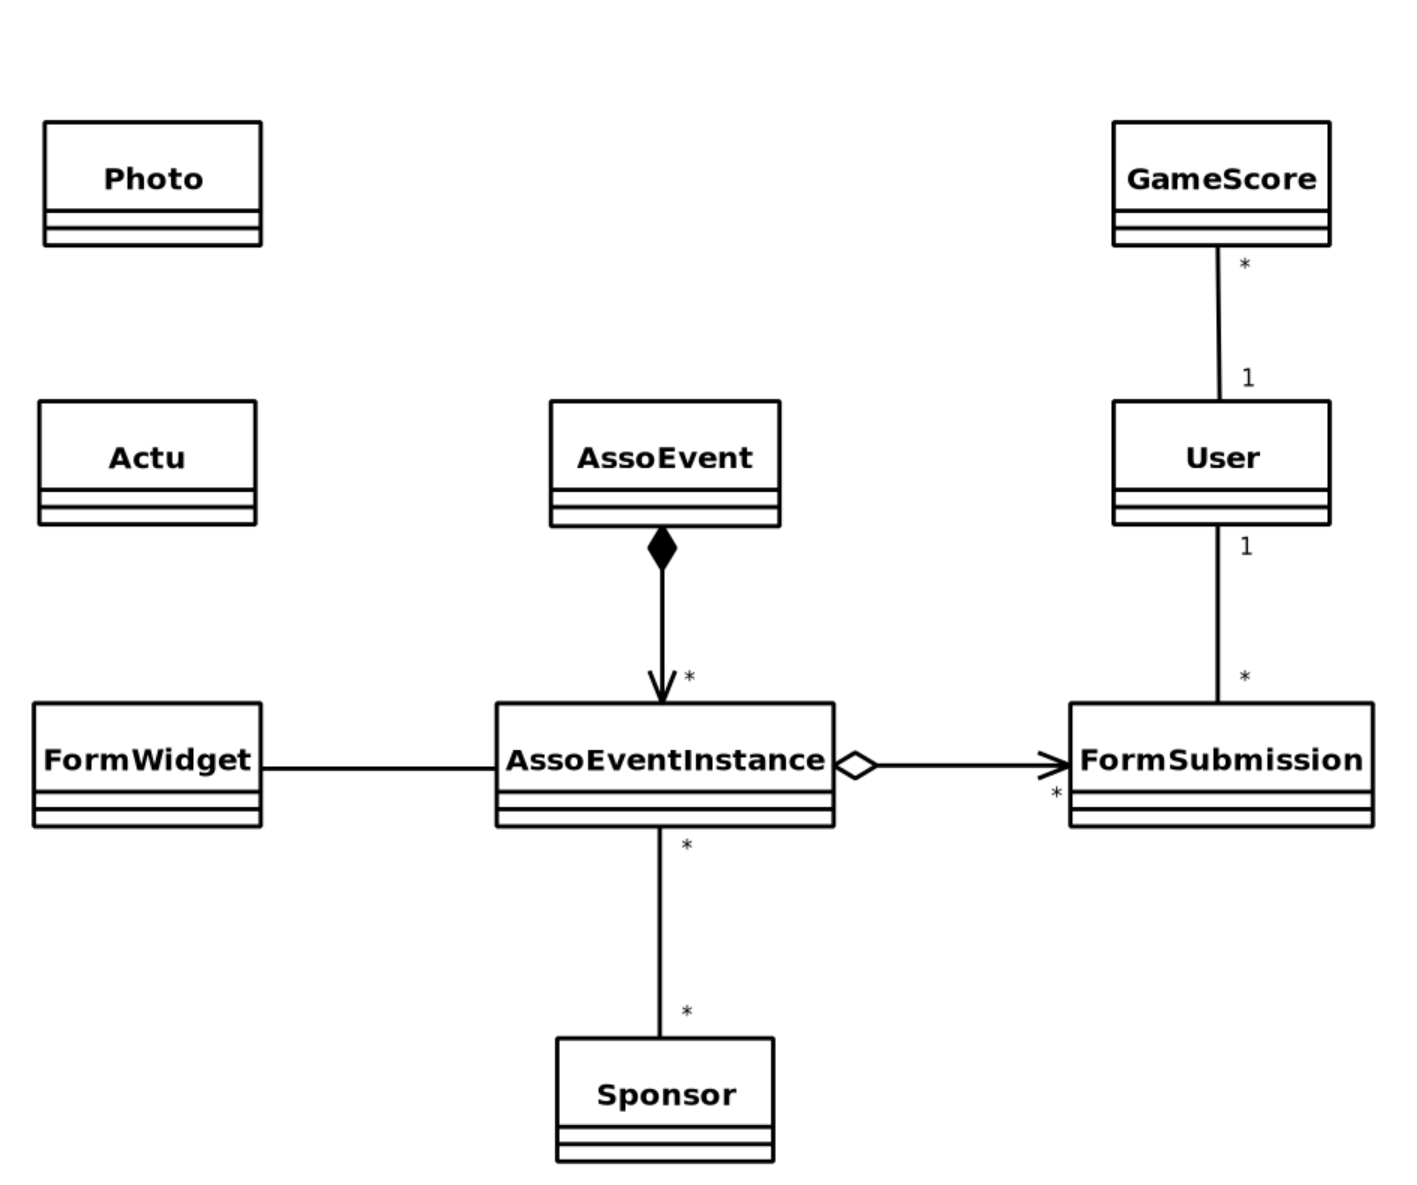
\includegraphics[width=0.8\textwidth]{pictures/database.png}
    \end{figure}
\end{frame}


% démonstration
% @Antoine
\section{Démonstration}
\sectitle{Démonstration du site web}

% conclusion
% @Antoine
\section{Conclusion}
\sectitle{Conclusion}

\begin{frame}
    \frametitle{Conclusion}
    \centering
    \textbf{Bilan}: Première version fontionnelle du site, sécurisée, adaptée aux besoins de l’association
    \vspace{1cm}

    \textbf{Ajout}: jeu OFNIvaders
    \vspace{1cm}

    \textbf{Pistes d'améliorations}: CMS, calendrier interactif, SEO, etc.
\end{frame}

\begin{frame}[plain, noframenumbering]
    \scshape\huge\centering
    \vspace{1cm}
    Merci pour votre attention !\par
    \vspace{2cm}
    Avez-vous des questions ?\par
\end{frame}


\end{document} 
